\documentclass[11pt]{article}
\usepackage{geometry,marginnote} % Pour passer au format A4
\geometry{hmargin=1cm, vmargin=1cm} % 

% Page et encodage
\usepackage[T1]{fontenc} % Use 8-bit encoding that has 256 glyphs
\usepackage[english,french]{babel} % Français et anglais
\usepackage[utf8]{inputenc} 

\usepackage{lmodern,numprint}
\setlength\parindent{0pt}

% Graphiques
\usepackage{graphicx,float,grffile,units}
\usepackage{tikz,pst-eucl,pst-plot,pstricks,pst-node,pstricks-add,pst-fun,pgfplots} 

% Maths et divers
\usepackage{amsmath,amsfonts,amssymb,amsthm,verbatim}
\usepackage{multicol,enumitem,url,eurosym,gensymb,tabularx}

\DeclareUnicodeCharacter{20AC}{\euro}



% Sections
\usepackage{sectsty} % Allows customizing section commands
\allsectionsfont{\centering \normalfont\scshape}

% Tête et pied de page
\usepackage{fancyhdr} \pagestyle{fancyplain} \fancyhead{} \fancyfoot{}

\renewcommand{\headrulewidth}{0pt} % Remove header underlines
\renewcommand{\footrulewidth}{0pt} % Remove footer underlines

\newcommand{\horrule}[1]{\rule{\linewidth}{#1}} % Create horizontal rule command with 1 argument of height

\newcommand{\Pointilles}[1][3]{%
  \multido{}{#1}{\makebox[\linewidth]{\dotfill}\\[\parskip]
}}

\newtheorem{Definition}{Définition}

\usepackage{siunitx}
\sisetup{
    detect-all,
    output-decimal-marker={,},
    group-minimum-digits = 3,
    group-separator={~},
    number-unit-separator={~},
    inter-unit-product={~}
}

\setlength{\columnseprule}{1pt}

\begin{document}

\textbf{Nom, Prénom :} \hspace{8cm} \textbf{Classe :} \hspace{3cm} \textbf{Date :}\\
\vspace{-0.8cm}
\begin{center}
  \textit{If you do the work, you get rewarded. There are no shortcuts in life}  - \textbf{Michael Jordan}
\end{center}
\vspace{-0.8cm}

\subsection*{Question de cours :}
  \begin{enumerate}
    \item[1.] Le segment MN s'écrit : \dotfill 
    \item[2.] La droite AC s'écrit : \dotfill 
    \item[3.] La demi-droite FV commençant en F s'écrit : \dotfill 
  \end{enumerate}

  \subsection*{Ex 1 - Calculer}

  \begin{minipage}[t]{0.30\textwidth}
    \begin{enumerate}
      \item[1.] Calculer AB. \\ \Pointilles[3]
      \item[2.] On a ML = 13cm. \\ Calculer BN. \\    \Pointilles[4]
      \item[3.] Calculer $A_1 B_1$ \\    \Pointilles[4]
      \item[4.] Calculer $C_2 F_2$ \\    \Pointilles[4]
      \item[5.] On a AF = 44 cm. \\ Calculer CL.   \Pointilles[4]
      \item[6.] On a $AB = 10m$ et $CD = 2 \times AB$ \\ Calculer AD.  \Pointilles[5]
    \end{enumerate}
    \end{minipage}
    \begin{minipage}[t]{0.70\textwidth}
      \begin{figure}[H]
        \centering
        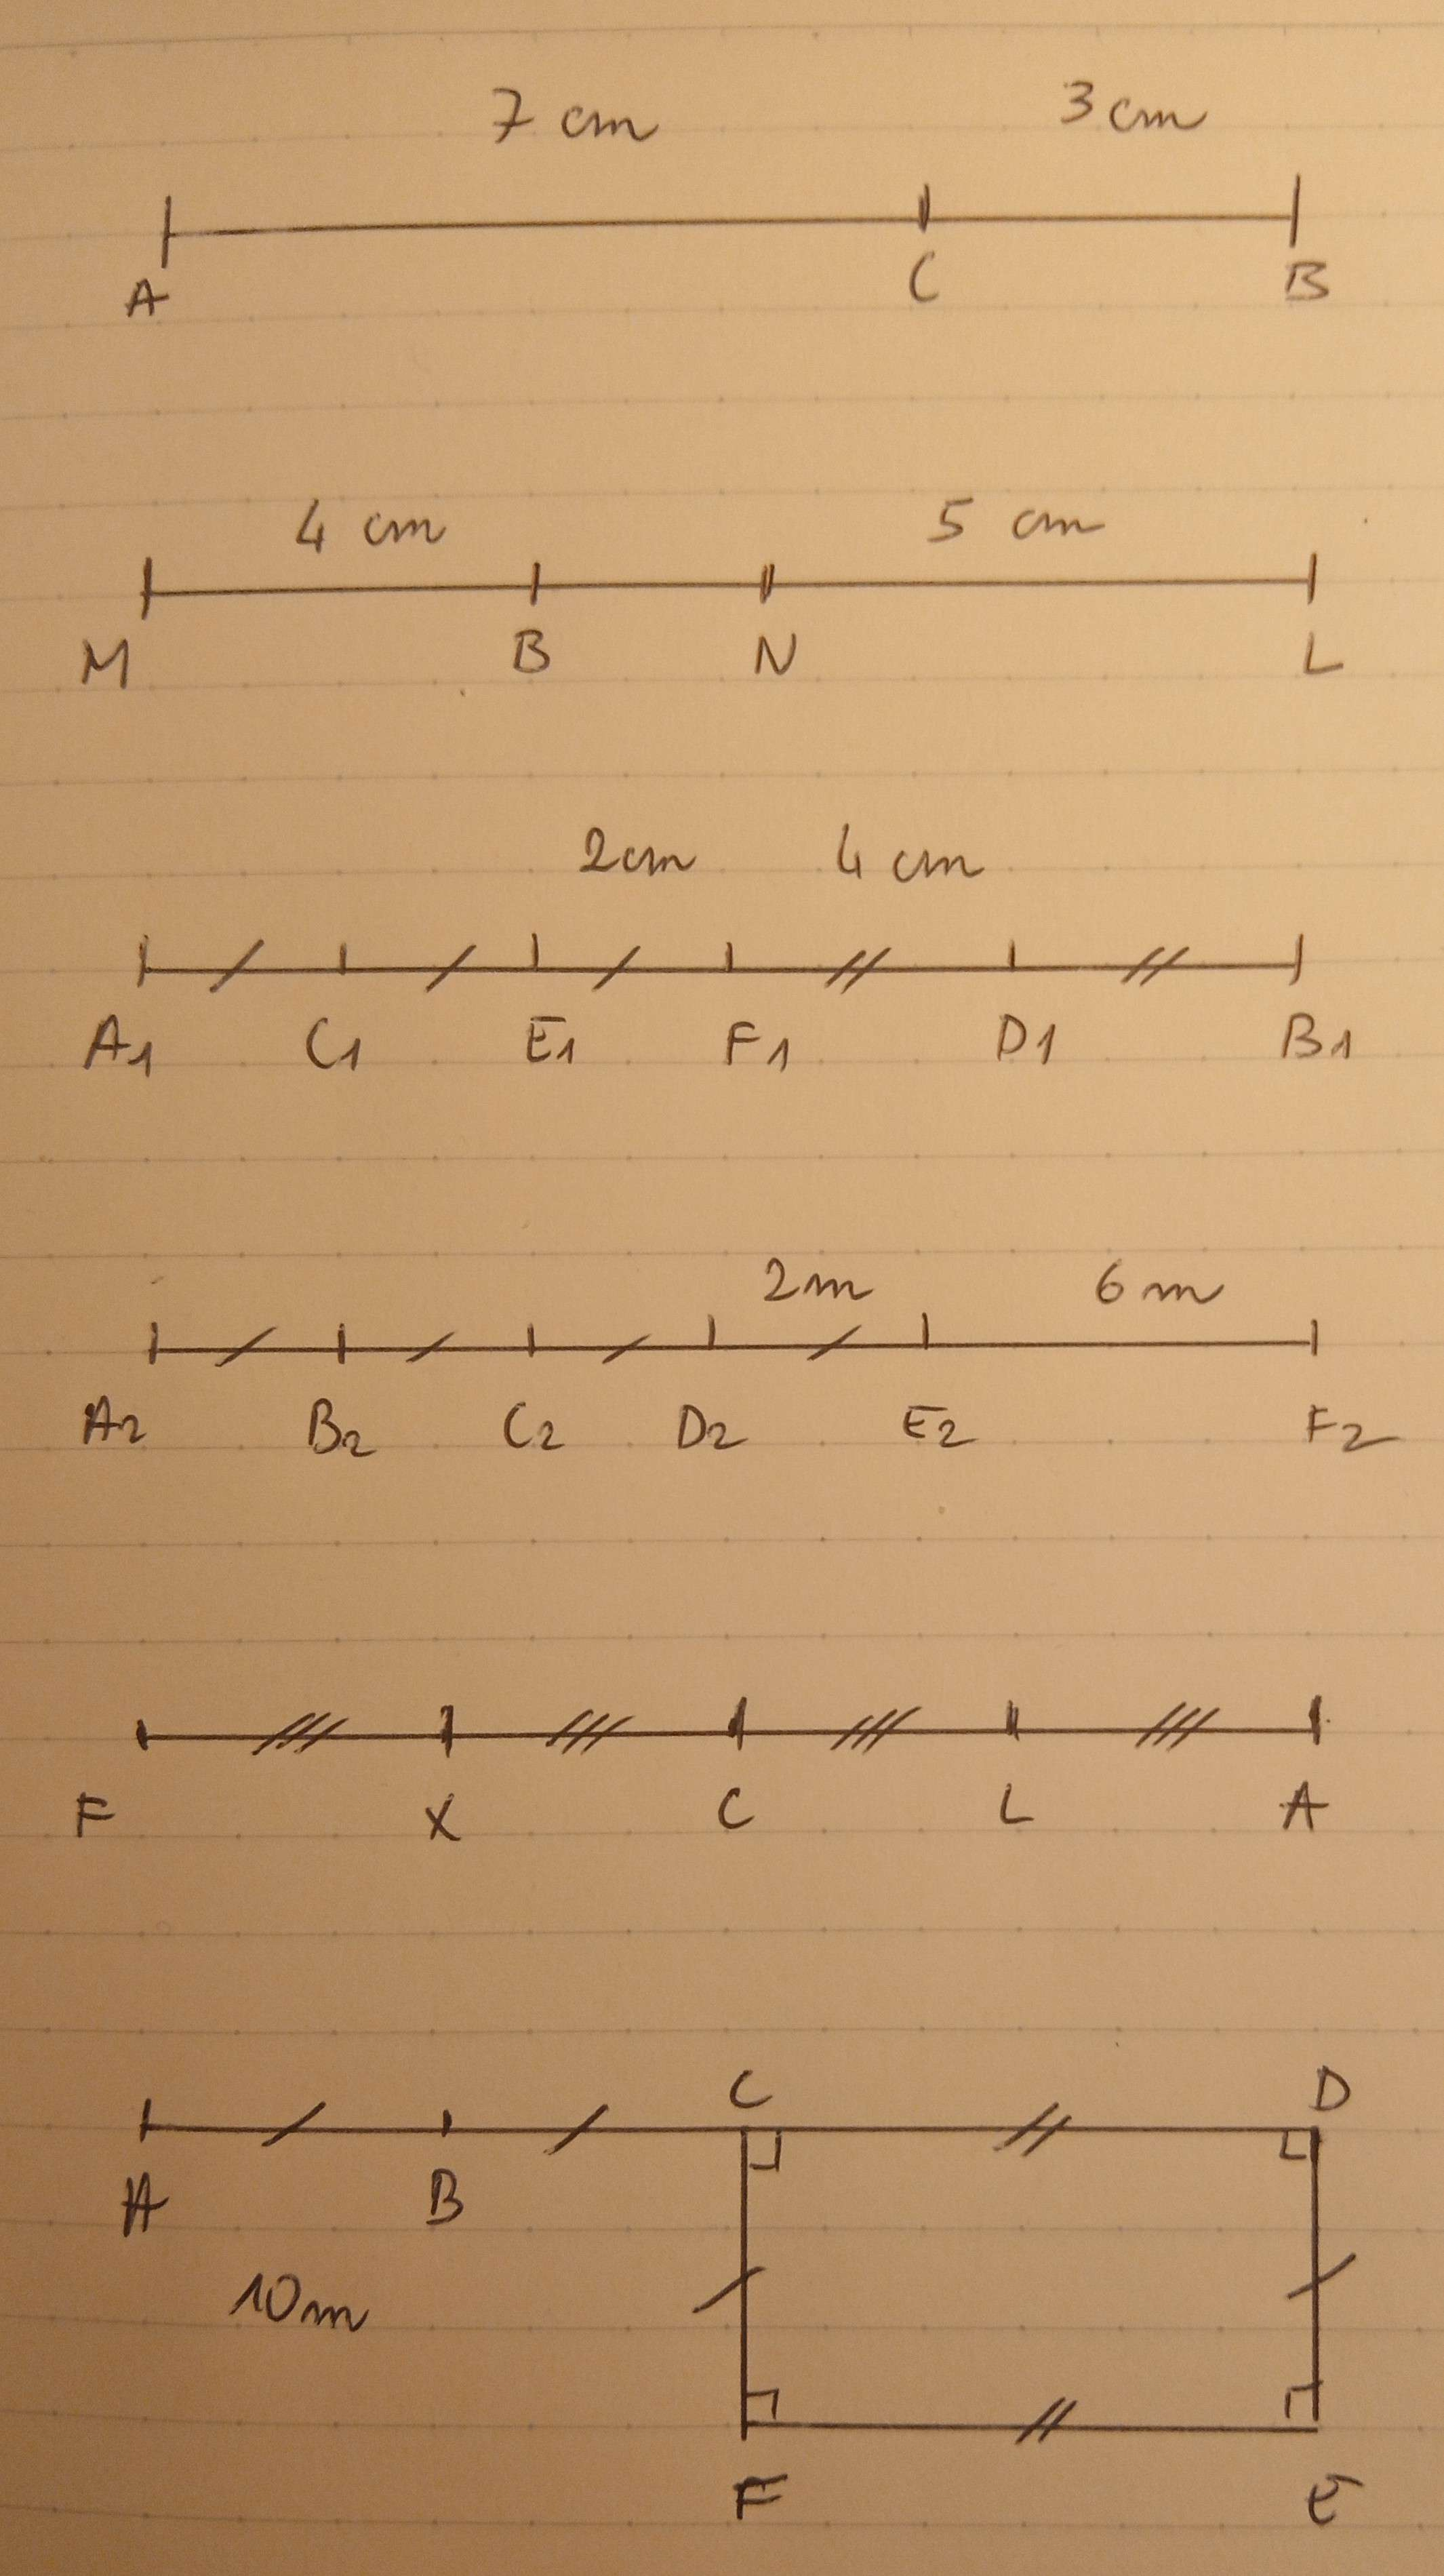
\includegraphics[width=0.8\linewidth]{6x4-geometrie-base/ex3.png}
      \end{figure}
    \end{minipage}

\newpage


\begin{minipage}[t]{0.25\textwidth}
\subsection*{Ex 2 - Tracer}

\begin{enumerate}
  \item[1.] 
  \begin{itemize}
    \item $[AB]$
    \item $(AC)$
    \item $(BC)$
  \end{itemize}
  \vspace{1.5cm}
  \item[2.] 
  \begin{itemize}
    \item $[A_1 B_1]$
    \item $[A_1 C_1)$
    \item $[A_1 D_1)$
    \item $(C_1D_1)$
  \end{itemize}
  \vspace{1.5cm}
  \item[3.] 
  \begin{itemize}
    \item RTYU est un rectangle\\
     avec RT = 3,2cm \\
     et TY = 4,6cm
    \item (RY)
  \end{itemize}
  \vspace{1cm}
  \item[] 
\end{enumerate}
\end{minipage}
\begin{minipage}[t]{0.75\textwidth}
  \vspace{-0.8cm}
  \begin{figure}[H]
    \centering
    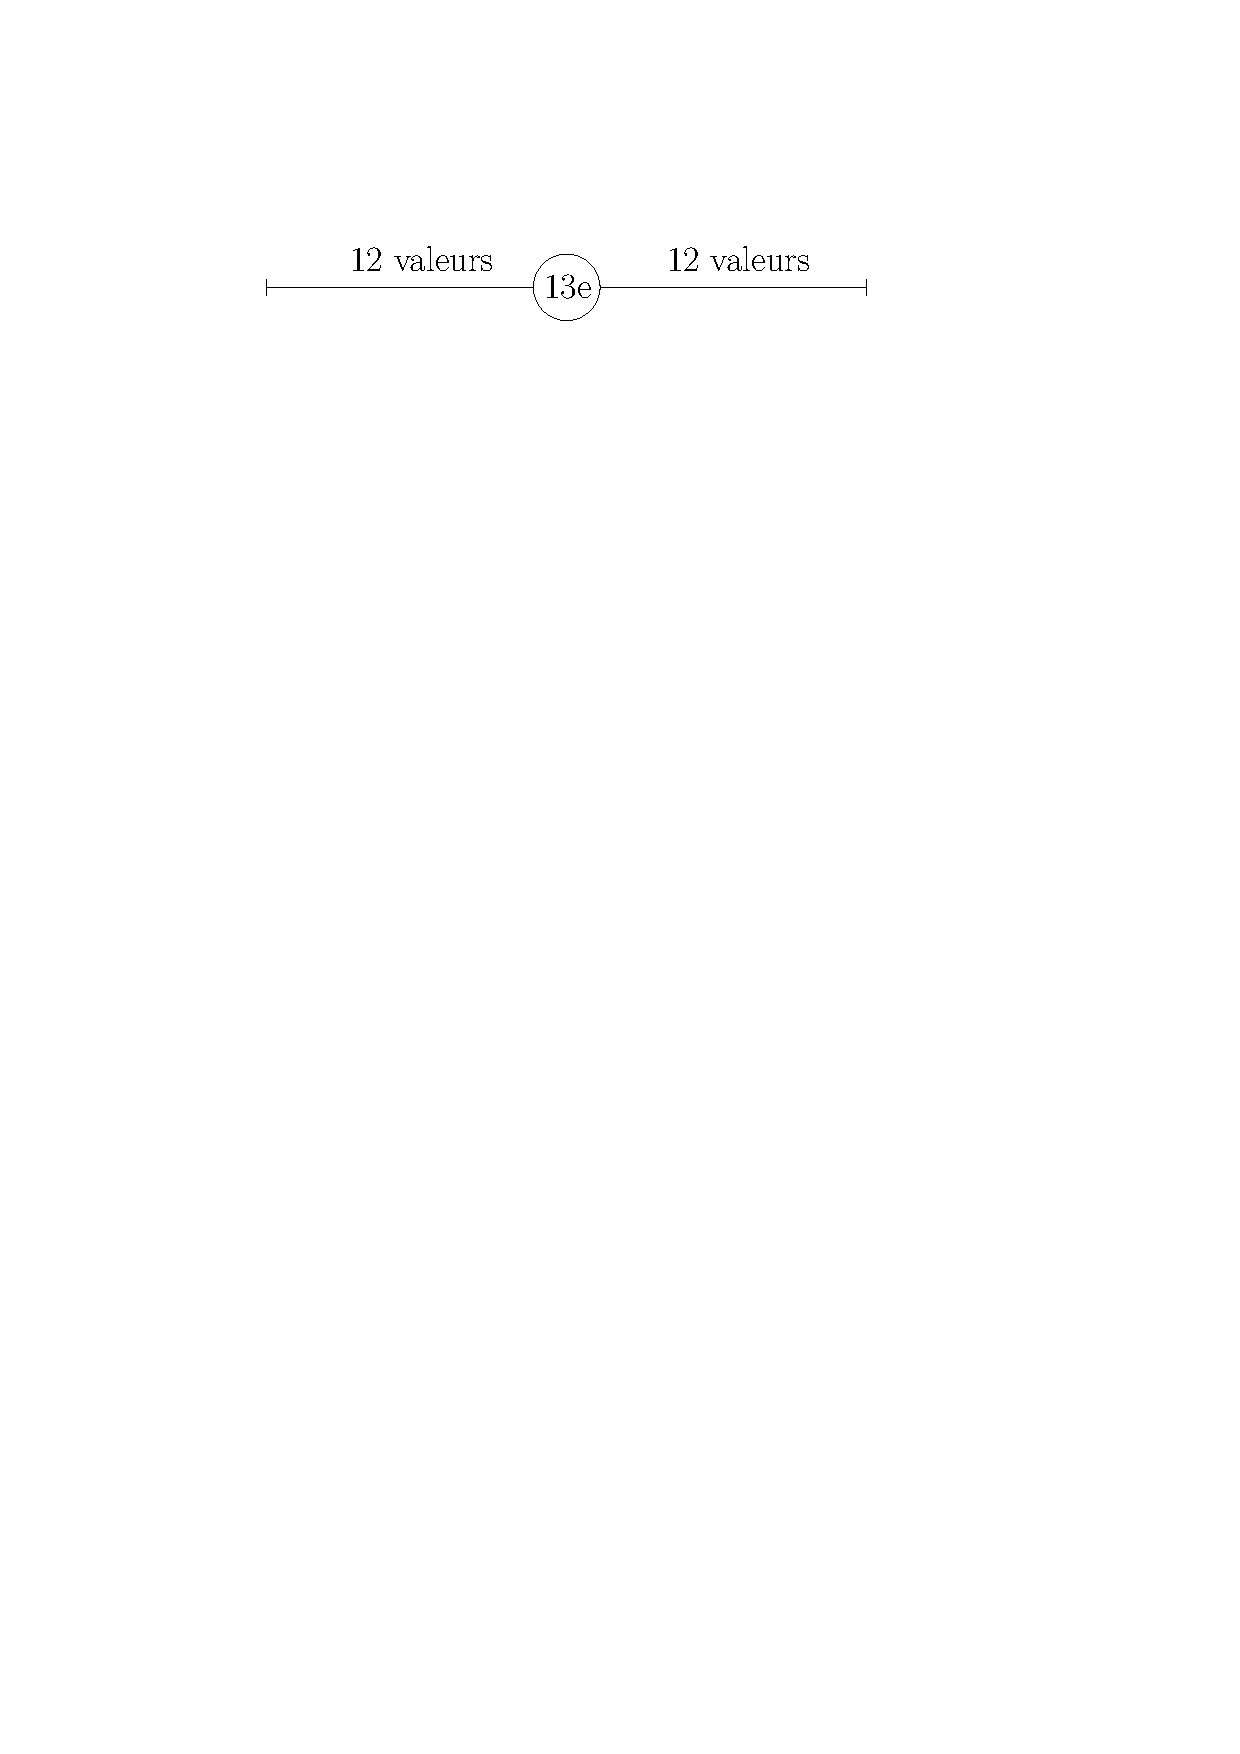
\includegraphics[width=0.5\linewidth]{6x4-geometrie-base/ex1.pdf}
  \end{figure}
  \vspace{-0.5cm}
  \begin{figure}[H]
    \centering
    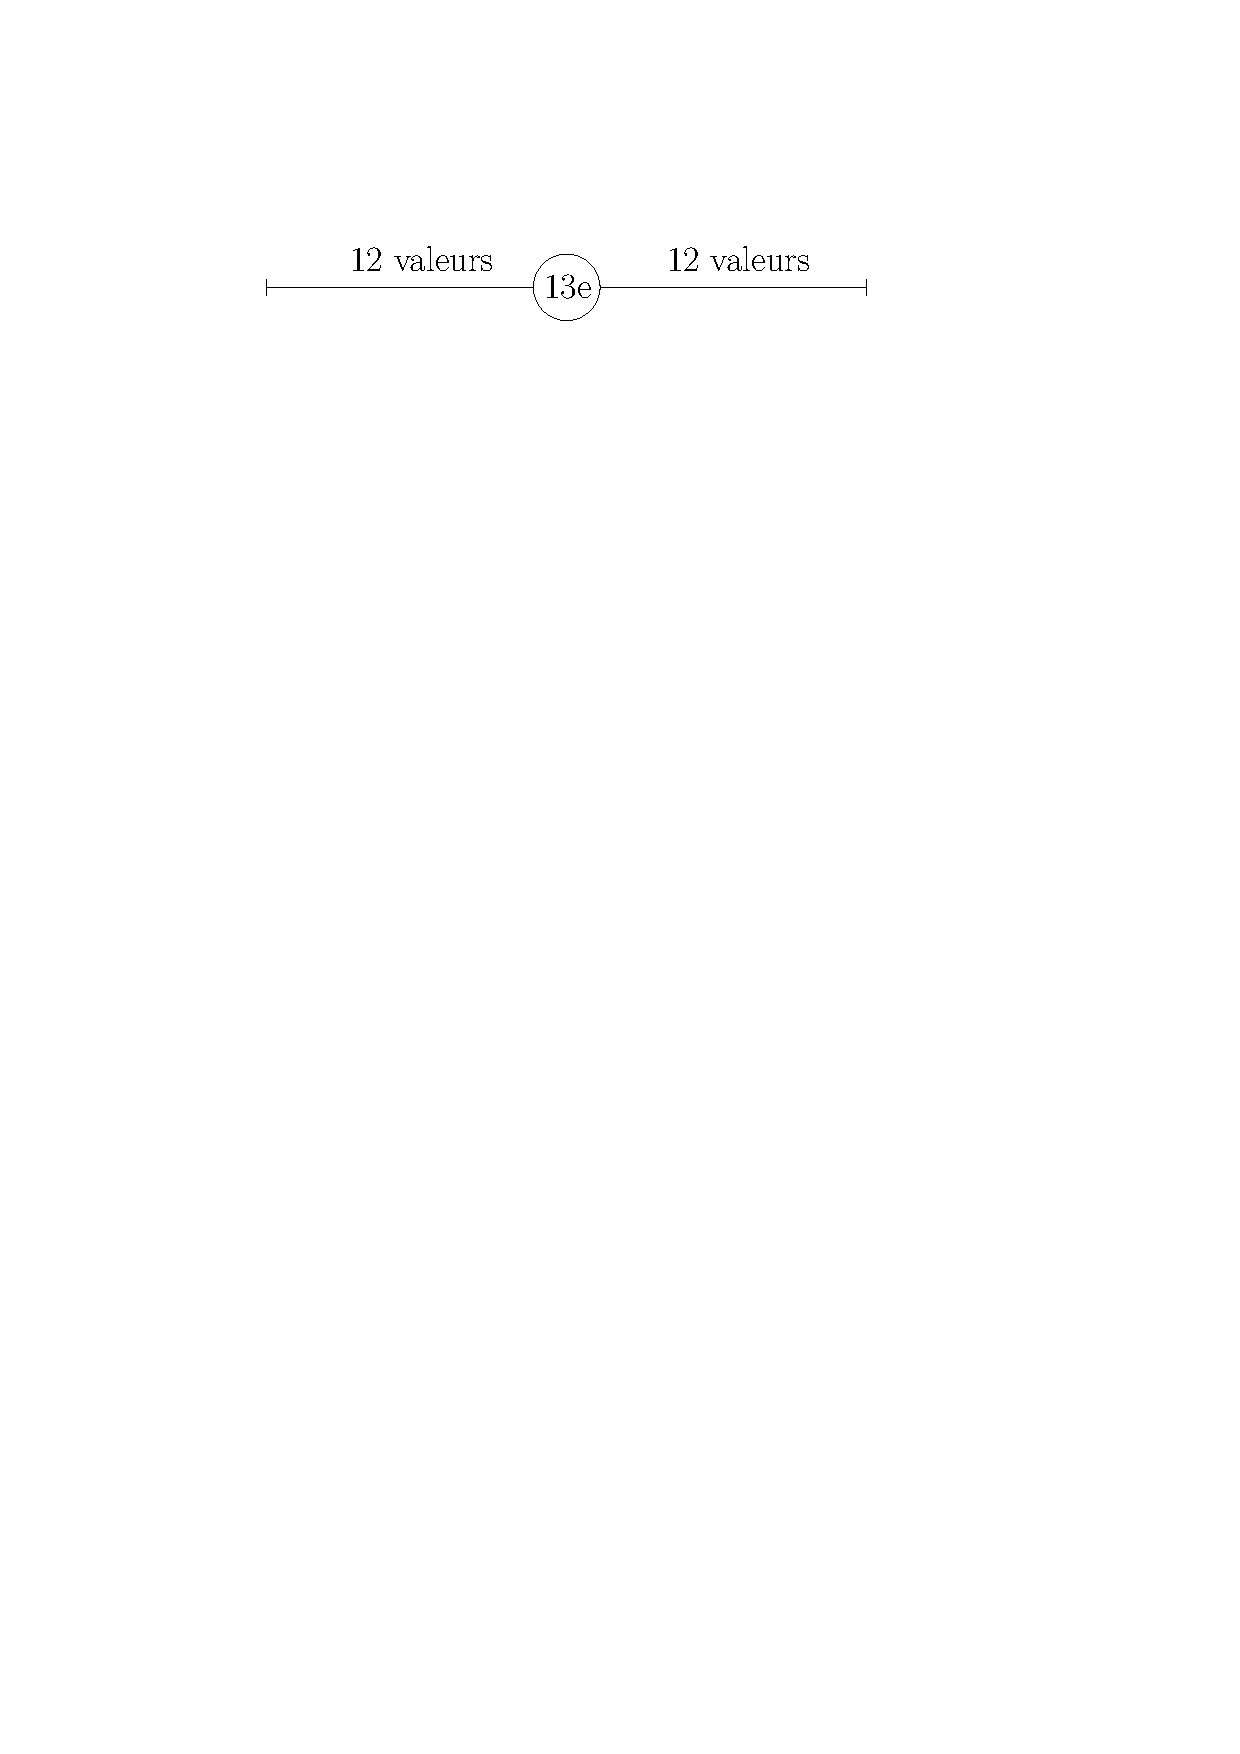
\includegraphics[width=0.5\linewidth]{6x4-geometrie-base/ex1.pdf}
  \end{figure}
  \vspace{-0.5cm}
  \begin{figure}[H]
    \centering
    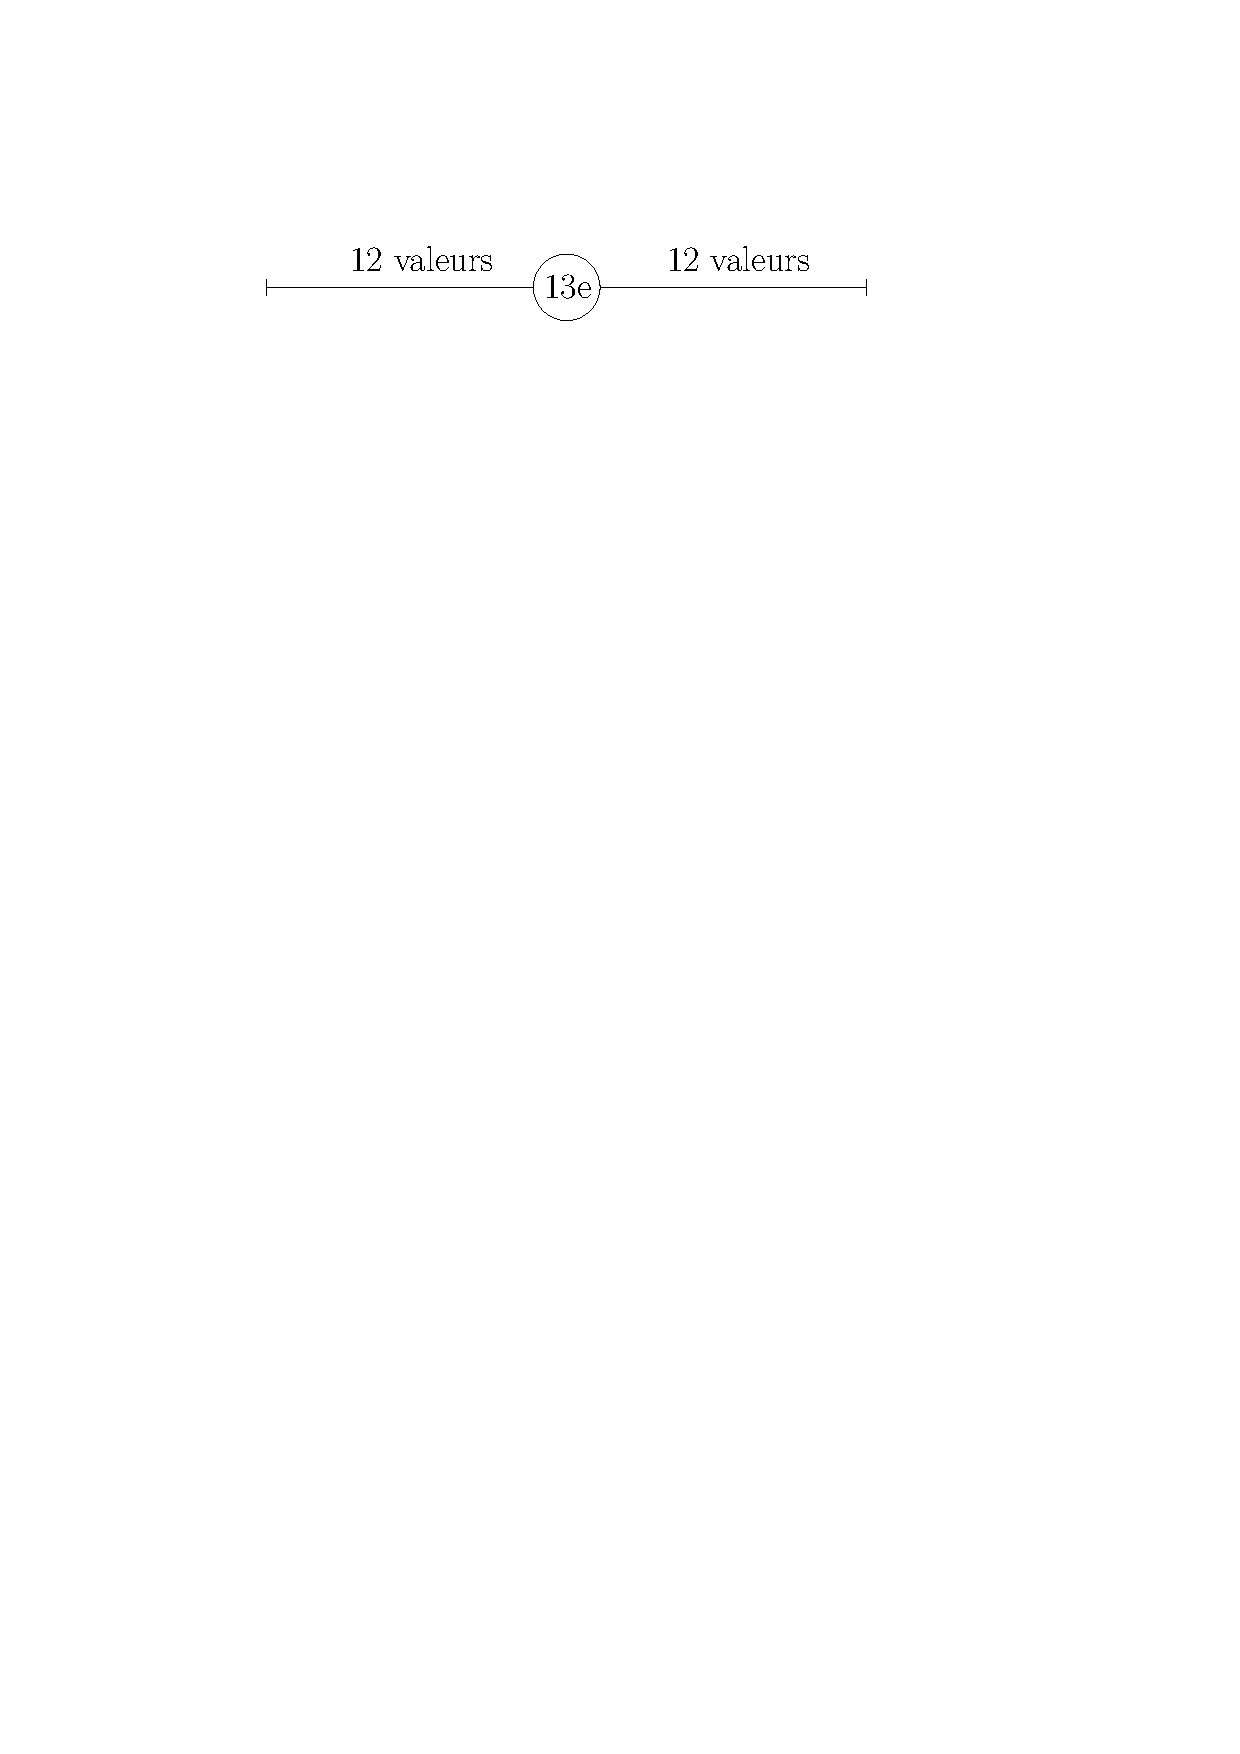
\includegraphics[width=0.5\linewidth]{6x4-geometrie-base/ex1.pdf}
  \end{figure}
\end{minipage}

\subsection*{Ex 3 - Mesurer}
\begin{minipage}[t]{0.50\textwidth}
\begin{enumerate}
  \item[1.] \dotfill \\
  \item[2.] \dotfill \\
  \item[3.] \dotfill \\
\end{enumerate}
\textbf{Pixel Art}
\end{minipage}
\begin{minipage}[t]{0.50\textwidth}
  \begin{figure}[H]
    \centering
    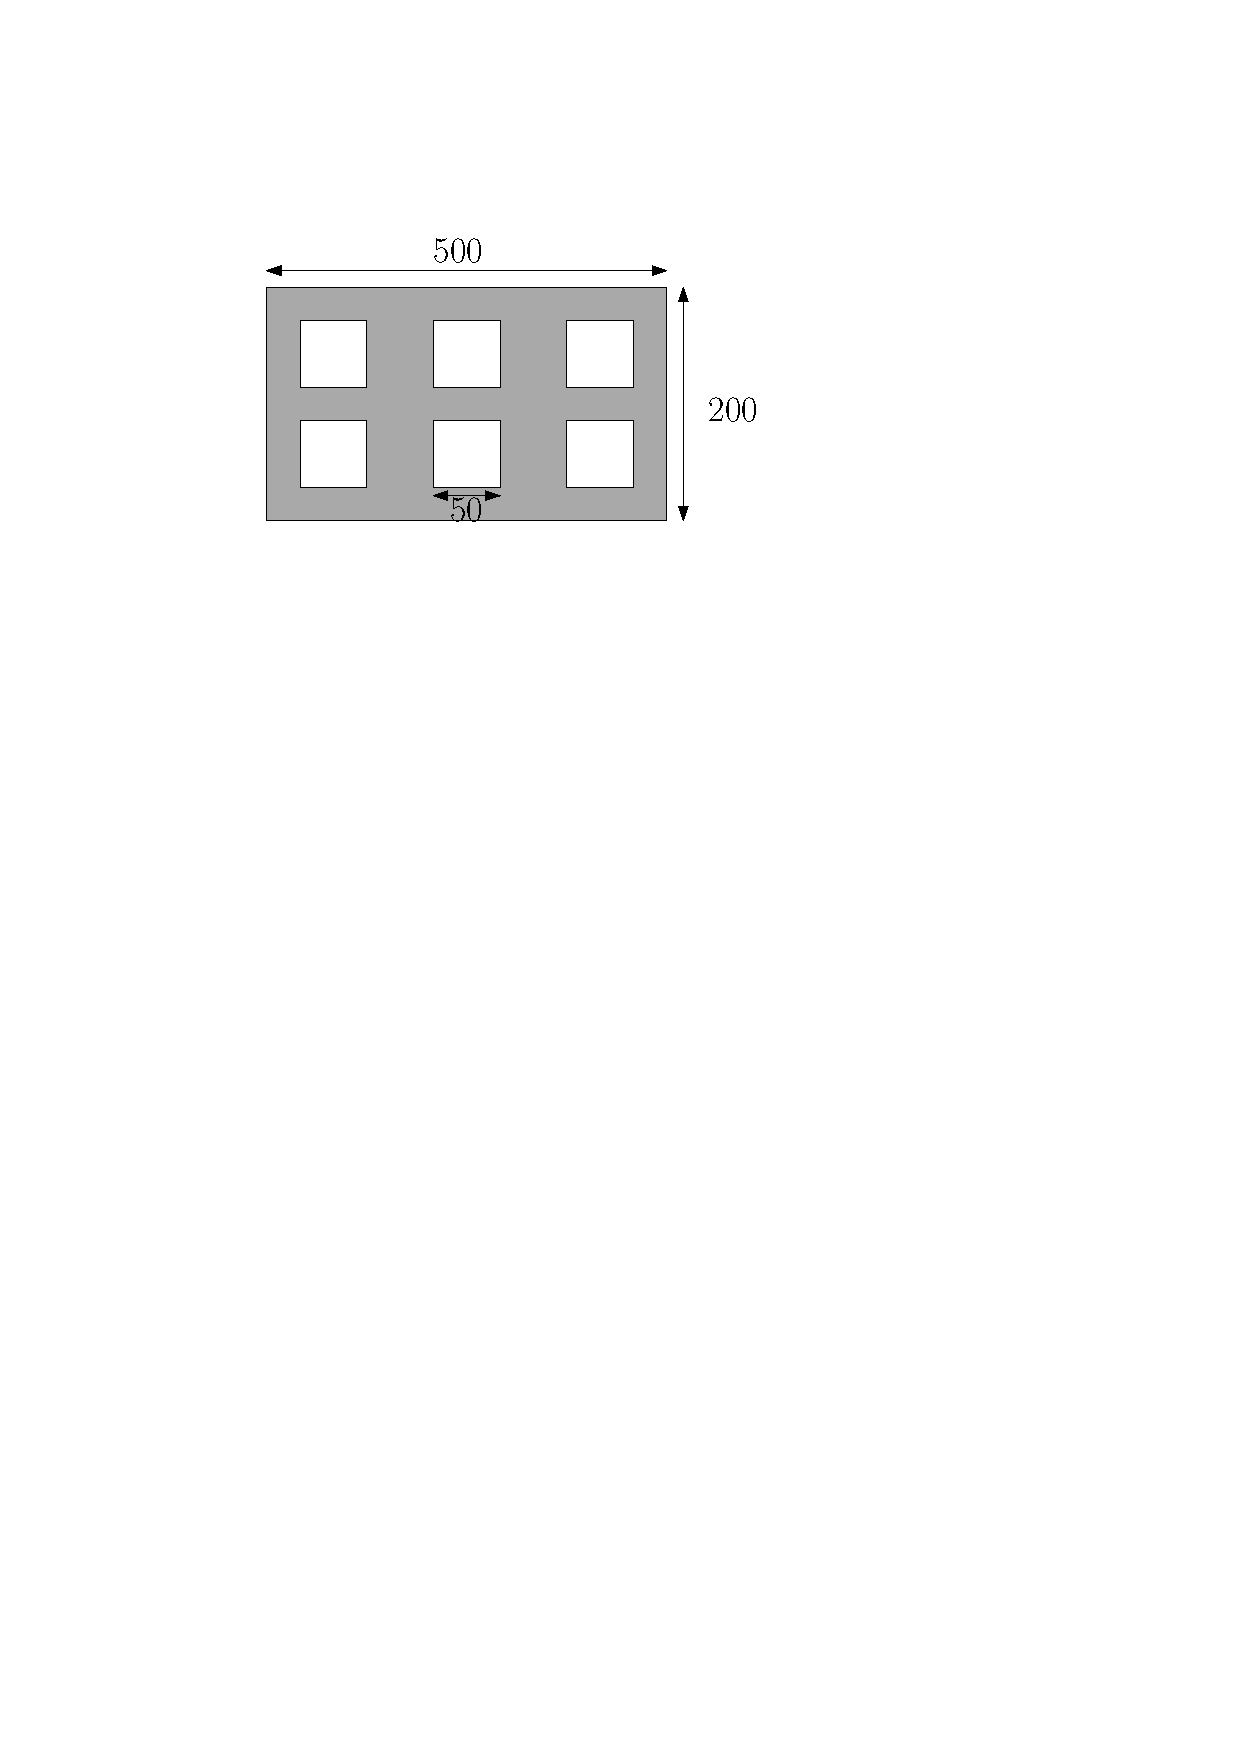
\includegraphics[width=0.8\linewidth]{6x4-geometrie-base/ex2.pdf}
  \end{figure}
\end{minipage}

\begin{minipage}[t]{0.50\textwidth}
\begin{figure}[H]
  \centering
  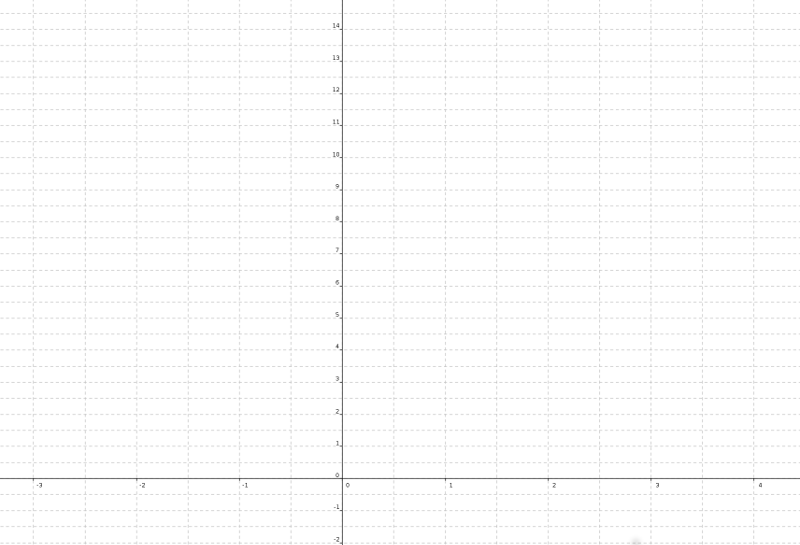
\includegraphics[width=0.8\linewidth]{6x4-geometrie-base/grille.png}
\end{figure}
\end{minipage}
\begin{minipage}[t]{0.50\textwidth}
  \begin{figure}[H]
    \centering
    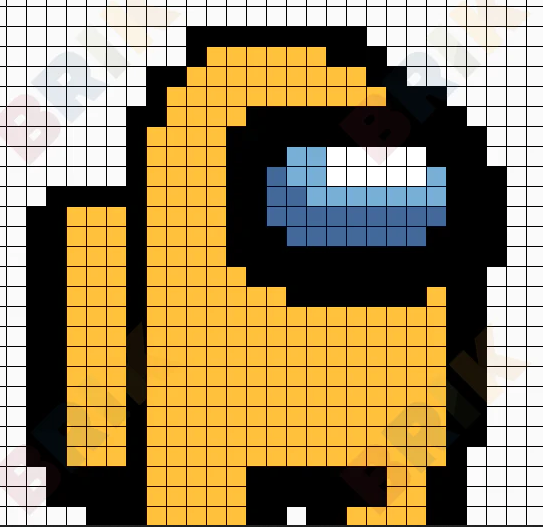
\includegraphics[width=0.8\linewidth]{6x4-geometrie-base/pa.png}
  \end{figure}
\end{minipage}
\end{document}